
%%%%%%%%%%%%%%%%%%%%%%%%%%%%%%%%%%%%%%%%%%%%%%%%%%%
\section{Architecture}
\label{sec:Architecture}
%%%%%%%%%%%%%%%%%%%%%%%%%%%%%%%%%%%%%%%%%%%%%%%%%%%


We now present the architectural specifications of \ac{bard}. The \ac{crisp} model described in Figure \ref{fig:crisp-dm} was used as a baseline to represent the data life cycle. \ac{bard} focuses on Data Quality (e.g.: cleaning, annotation), Data Representation (e.g.: anonymization, ciphering) and Data Processing (e.g.: computation on ciphertext).

The \emph{Data Quality} step refers to the transformation of raw input data into a structured, consistent, and, whenever possible, complete representation. An important aspect to mention in this step is that the data must be processed in plaintext by a trusted entity, meaning that this is done by the data owner or an entity in which the data owner trusts and has explicit permission to perform the operations.
The \emph{Data Representation} step refers to the protection of \ac{pii} contained in the data. This data should be: integrated using privacy-preserving data integration techniques; aggregated using anonymization techniques; and represented using either hashing techniques or homomorphic cryptosystems.
The \emph{Data Processing} step is done in two different approaches. On one hand, \ac{smpc} techniques, such as \ac{gc} or \ac{he}, are performed over the data. On the other hand, \ac{ml} algorithms, adapted to work with hashed or encrypted data, are used in performing knowledge learning.

We now describe the internal components of a \ac{bard} solution.
As stated in the objectives (Section \ref{sec:Objectives}), the main goal of \ac{bard} is to produce a platform that will provide mechanisms so that companies can perform privacy-preserving computations for \ac{ml} algorithms, that are respectful of user privacy, and comply with the legislation. A representation of a solution is described by the following components: 
\begin{itemize}
	\item \textbf{A dataset} to train the \ac{ml} algorithms, or the values representing the already trained algorithms.
	\item \textbf{A sample} or a set of samples that represent the user inputs, to be predicted.
	\item \textbf{Prediction algorithms} that depend on the \ac{ml} algorithms and the privacy-preserving techniques chosen.
	\item \textbf{A set of toolkits} for each of the techniques used.
\end{itemize}

These components altogether allow the user of the platform to perform \ac{ppml} over data of his own choosing.
In Figure \ref{fig:bard-architecture} we present the architecture for \ac{bard}. With it, we aim at providing companies a way to integrate their Big Data systems processes with privacy-preserving ML algorithms, allowing them to provide additional data privacy guarantees to their clients.

\begin{figure}[ht]
\centering
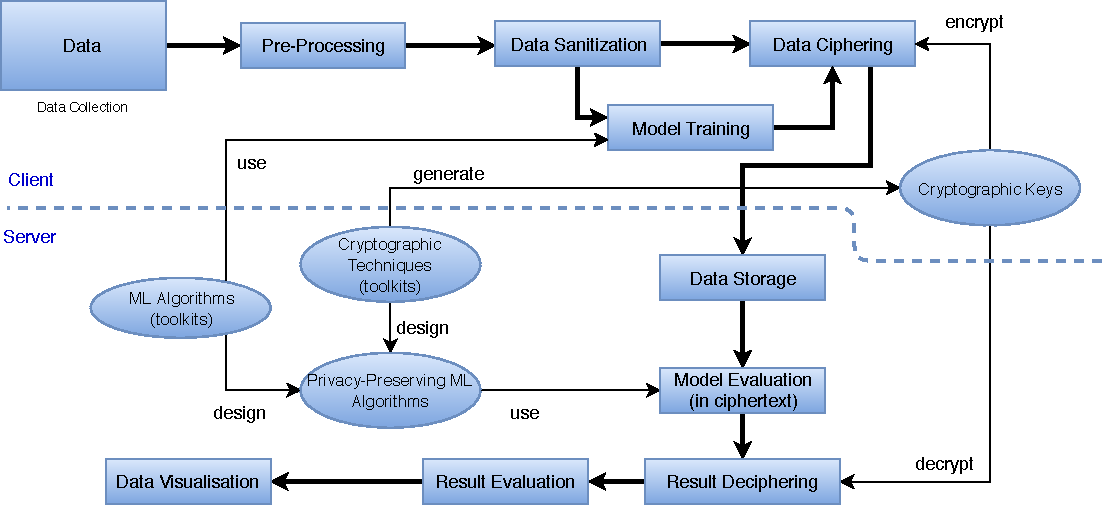
\includegraphics[width=1\textwidth]{images/BARDArchitecture.pdf}
\caption{Platform architecture for \acs{bard}.}
\label{fig:bard-architecture}
\end{figure}

We assume that only two parties exist: the client and the server. 
The client represents a user or an individual who owns the data and wishes to perform some processing over it. 
The server represents a cloud or service provider who has the computational capabilities and know-how to perform such processing.
The data are provided by the client in the form of a dataset. 
That dataset is then pre-processed and the data are sanitized, to remove outliers and missing values.
The model training is performed in the usual manner. 
The model evaluation process is the main focus of our work, and it is were the privacy-preserving techniques are deployed. 
In the end of the flow, the platform produces the prediction results.

%%%%%%%%%%%%%%%%%%%%%%%%%%%%%%%%%%%%%%%%%%%%%%%%%%%
\section{Our Contributions to BARD}
\label{sec:MyContributions}
%%%%%%%%%%%%%%%%%%%%%%%%%%%%%%%%%%%%%%%%%%%%%%%%%%%

Our contributions to \ac{bard} project were the development of a solution using the toolkit VIPP for privacy-preserving computations using \ac{gc}. This includes the development of a baseline system, the adapted algorithms, the testing of the various toolkits and the actual development of the final solution with \ac{gc}.

As mentioned in Section \ref{sec:Intro_Contributions}, this work is part of a project, and the development of the solution was done by a team. Some of the results shown in this dissertation are presented for completeness only, as they were developed by the \ac{bard} team at Altran. Those results are presented in Sections \ref{ssec:exec_he_lr} and \ref{ssec:exec_he_svm}, for the results obtained using \ac{he} and \ac{lr}, and for the results using \ac{he} and \ac{svm}, respectively, and Sections \ref{ssec:comm_phe} and \ref{ssec:comm_fhe} for the communication costs of using \ac{phe} and \ac{fhe}. All the remaining results were obtained by the author of this dissertation.
